\documentclass[11pt,letterpaper]{article}
\usepackage[T1]{fontenc}
\usepackage{lmodern,microtype,amsmath,amssymb,graphicx,booktabs,tabularx,array,enumitem,xcolor,fancyhdr,titlesec,tcolorbox,caption}
\tcbuselibrary{breakable}
\usepackage[margin=.8in,headheight=15pt,headsep=18pt,footskip=25pt]{geometry}
\usepackage[colorlinks=true,urlcolor=teal,linkcolor=olive]{hyperref}
\definecolor{olive}{HTML}{536240}\definecolor{ink}{HTML}{293329}\definecolor{teal}{HTML}{17677A}\definecolor{gold}{HTML}{A55C21}\definecolor{soft}{HTML}{EEF3E8}\definecolor{warm}{HTML}{FBEFDF}
\color{ink}\setlength{\parindent}{0pt}\setlength{\parskip}{7pt}
\setlist{leftmargin=1.4em,itemsep=3pt,topsep=3pt}
\renewcommand{\thesection}{8.\arabic{section}}
\titleformat{\section}{\Large\bfseries\color{olive}}{\thesection}{.6em}{}
\titleformat{\subsection}{\large\bfseries\color{teal}}{}{0pt}{}
\titlespacing*{\section}{0pt}{4pt}{12pt}\titlespacing*{\subsection}{0pt}{11pt}{4pt}
\pagestyle{fancy}\fancyhf{}\fancyhead[L]{\small\sffamily MATH\& 107 / WEEK 8 / PART II}\fancyhead[R]{\small\sffamily Best Choices and Linear Programming}\fancyfoot[L]{\small\sffamily Math in Society / Dr Lee}\fancyfoot[R]{\small\sffamily\thepage}\renewcommand{\headrulewidth}{.3pt}
\tcbset{boxrule=.5pt,arc=2mm,left=10pt,right=10pt,top=7pt,bottom=7pt,before skip=9pt,after skip=9pt,colframe=olive!35,colback=soft,fonttitle=\bfseries,coltitle=teal,colbacktitle=soft}
\newcolumntype{Y}{>{\raggedright\arraybackslash}X}
\captionsetup{font=small,labelformat=empty,textfont={color=teal},skip=7pt}
\hypersetup{pdftitle={Week 8, Part II: Best Choices and Linear Programming},pdfauthor={MATH and 107 / Dr Lee}}
\usepackage{needspace}
\pdfinfoomitdate=1
\pdftrailerid{}
\pdfsuppressptexinfo=15
\setlength{\emergencystretch}{2em}

\begin{document}
\setcounter{section}{5}
{\small\sffamily\color{olive}WEEK 8 / PART II / LINEAR PROGRAMMING\par}
\vspace{10pt}
{\fontsize{31}{35}\selectfont\bfseries\color{olive}Which plan is best?\par}
\vspace{8pt}
{\large Keep the allowable choices fixed, state a goal, and compare the consequences. A mathematical optimum answers the question you actually put into the model.\par}
\begin{center}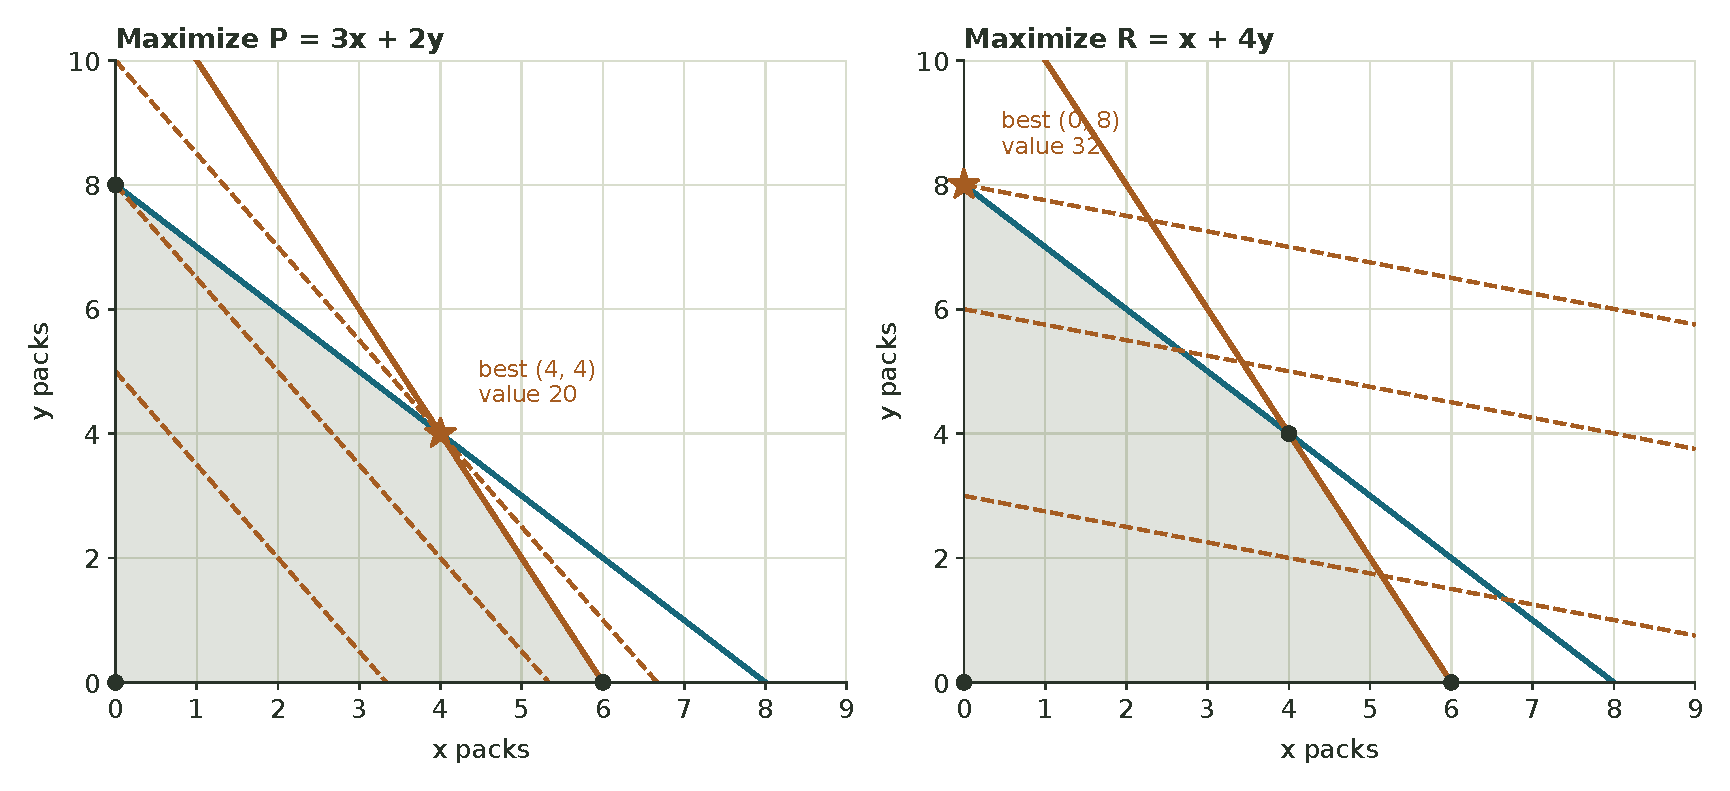
\includegraphics[width=\linewidth]{../assets/week8/objective-levels.pdf}\end{center}
\begin{tcolorbox}[title={From geometry to a decision}]
The club's feasible region has corners $(0,0),(6,0),(4,4),(0,8)$. With contribution $P=3x+2y$, four packs of each type give the largest total. A different goal can choose a different corner, or leave an entire edge tied.
\end{tcolorbox}
Part I developed the variables, inequalities, and feasible geometry. Part II combines them with an objective. We study maximum and minimum values, tied solutions, infeasible models, unbounded scores, and whole-number restrictions. Worked examples and review solutions show how to verify each conclusion.

For the core method you need only substitution and comparison. Equal-score lines and convex mixtures explain why the method works. The whole-number investigation is an extension.

\medskip
\href{https://bobovski66.github.io/MathInSociety/readings/week8_reading.html}{Online reading}\quad\textperiodcentered\quad\href{https://bobovski66.github.io/MathInSociety/demos/linear_programming.html}{Optimizer}\quad\textperiodcentered\quad\href{https://bobovski66.github.io/MathInSociety/labs/week8_optimization_lab.html}{Optimization extension}

\clearpage


\Needspace{6\baselineskip}\section{An objective gives each plan a score}

The club earns a \$3 contribution from each type-A pack and \$2 from each type-B pack. Its total contribution is

\[P=3x+2y.\]
This is the \emph{objective function}: a rule assigning a number to each plan. The letter P names the total contribution in dollars. To \emph{maximize} it means to find the largest value among feasible plans.


\begin{tcolorbox}[title={Example \textperiodcentered{} Feasible does not mean optimal},breakable]

The feasible plan (3,3) gives \(P=3(3)+2(3)=15\) dollars. The feasible plan (4,4) gives \(P=3(4)+2(4)=20\) dollars. So (3,3) is possible but does not give the largest contribution.


The infeasible plan (5,3) would give \$21. That larger score does not make it an allowable choice: it exceeds the ingredient supply. We optimize \emph{within} the feasible region.


\end{tcolorbox}

A function such as \(3x+2y\) is \emph{linear}: each extra unit of x adds the same amount, and each extra unit of y adds the same amount. There is no product \(xy\), squared quantity, or changing rate. A \emph{linear program} combines a linear objective with linear constraints. ``Programming'' here means planning or optimization; writing computer code is not required.



\begin{tcolorbox}[title={Pause and try 1},breakable]
At (2,5), what is P=3x+2y? Does the value alone tell you the plan is feasible?
\end{tcolorbox}


\Needspace{6\baselineskip}\section{For this bounded polygon, compare the corners}

Our continuous feasible region contains infinitely many points. The \emph{corner-point principle} says that a linear objective on a nonempty, closed, bounded polygonal feasible region attains its maximum and minimum at vertices. ``Bounded'' means it fits inside some finite box. ``Closed'' here means the boundary is included.


This guarantees that at least one vertex gives the best value. It does not guarantee a unique best point, or say that every best point must be a vertex. Those distinctions matter when there is a tie.



\par\medskip{\small\renewcommand{\arraystretch}{1.35}\begin{tabularx}{\linewidth}{@{}YYY@{}}\toprule
Feasible vertex & Calculation of P = 3x + 2y & Contribution\\
\midrule
(0,0) & 3(0)+2(0) & \$0\\
(6,0) & 3(6)+2(0) & \$18\\
(4,4) & 3(4)+2(4) & \$20\\
(0,8) & 3(0)+2(8) & \$16\\
\bottomrule\end{tabularx}}\par\medskip


The largest entry is \$20 at (4,4). The recommendation is to make \emph{four of each type}, with contribution \emph{\$20}. Report both the plan and its value; they answer different parts of the question.


\begin{tcolorbox}[title={Why a corner comparison can work},breakable,colback=warm,colbacktitle=warm,coltitle=gold,colframe=gold!35]

Any point in a filled convex polygon can be expressed as a mixture of its vertices. A linear objective at that point is the same mixture of the vertex scores. An average of scores cannot exceed the largest score or fall below the smallest. This is the geometric reason the table can locate an optimum.


\end{tcolorbox}


\par\medskip\noindent\begin{minipage}{\linewidth}
\centering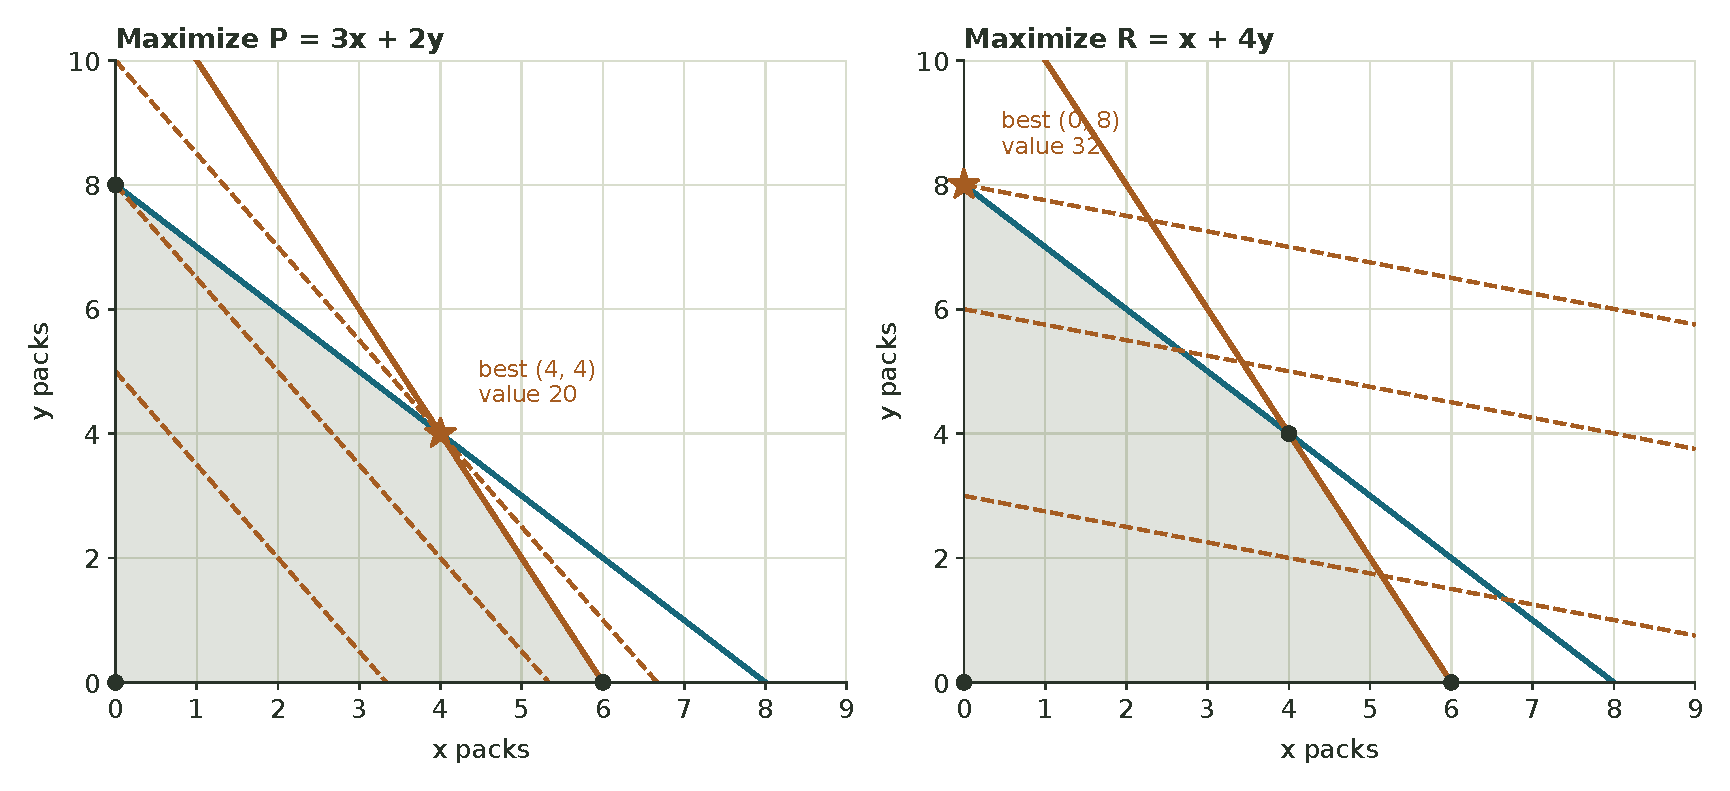
\includegraphics[width=\linewidth,height=3.2in,keepaspectratio]{../assets/week8/objective-levels.pdf}
\captionof*{figure}{Each dashed line joins plans with an equal objective value. Moving to a parallel line changes that score, not the resource constraints. The star marks the last feasible contact in the direction of increasing score.}
\end{minipage}\par\medskip


In our model, the best plan is also a whole-number plan, so it remains optimal if we restrict production to whole packs. A continuous optimum is an upper bound for the integer choices; when a whole-number plan attains it, the integer problem is solved too.



\begin{tcolorbox}[title={Pause and try 2},breakable]
Why is checking just the two axis corners insufficient?
\end{tcolorbox}


\Needspace{6\baselineskip}\section{The feasible region stays; the goal can change}

Suppose a new contribution schedule favors type B, with objective \(R=x+4y\). At the same four vertices its values are 0, 6, 20, and 32. Now (0,8) is best. The resource limits and region did not change. The objective changed.


Alternatively, suppose the club wants the largest \emph{number of packs}, regardless of type. Maximize \(T=x+y\). The packing limit already tells us \(T\leq8\). Both (4,4) and (0,8) attain 8, and every point on the segment between them also attains 8.



\par\medskip\noindent\begin{minipage}{\linewidth}
\centering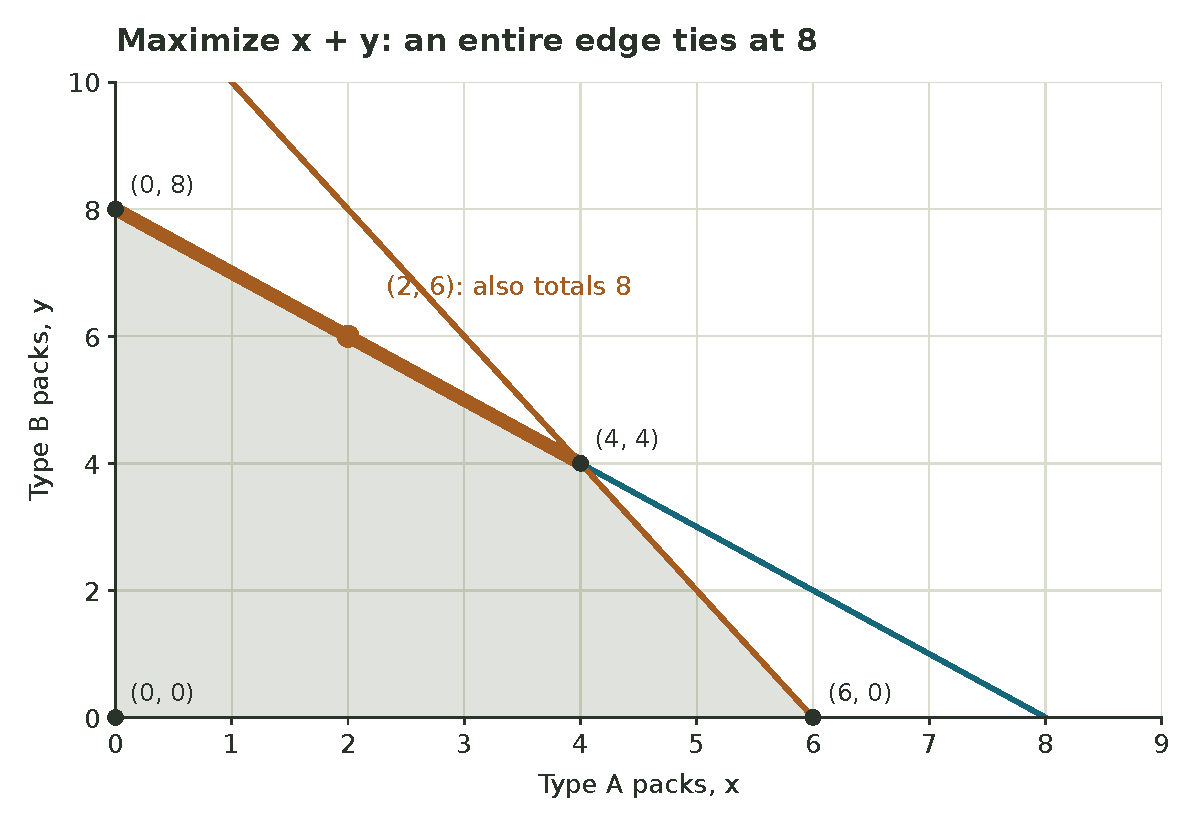
\includegraphics[width=\linewidth,height=3.2in,keepaspectratio]{../assets/week8/optimal-edge.pdf}
\captionof*{figure}{These are multiple optimal solutions. If actual packs must be whole, the five plans (0,8), (1,7), (2,6), (3,5), and (4,4) all attain the same largest total.}
\end{minipage}\par\medskip


\begin{tcolorbox}[title={Example \textperiodcentered{} A tie leaves room for another consideration},breakable]

Under the objective ``make as many packs as possible,'' (4,4) and (0,8) are equally good. Their ingredient use differs: 12 portions versus 8. If the club also wants to save ingredients among tied plans, it can choose (0,8). If it wants the larger contribution among those tied plans, it can choose (4,4).


A second goal can distinguish plans that tie under the first. We should name that goal rather than pretend the first objective made the whole decision.


\end{tcolorbox}


\begin{tcolorbox}[title={Pause and try 3},breakable]
If two adjacent feasible vertices both give the maximum score for a linear objective, what happens between them? Does the same conclusion follow merely because two vertices have equal scores?
\end{tcolorbox}

\clearpage

\Needspace{6\baselineskip}\section{``At least'' often reverses the feasible side}

An invented supply order offers two bundles. Bundle A contains 1 notebook and 2 pencils and costs \$4. Bundle B contains 1 notebook and 1 pencil and costs \$3. We need at least 6 notebooks and at least 8 pencils. Let x and y be the respective bundle counts.

\[x+y\geq6,\qquad 2x+y\geq8,\qquad x,y\geq0;\qquad \text{minimize }C=4x+3y.\]
We can buy extra supplies, so there is no upper limit in this model. The feasible region extends up and to the right. It is \emph{unbounded}, but that does not mean its minimum cost is missing.



\par\medskip\noindent\begin{minipage}{\linewidth}
\centering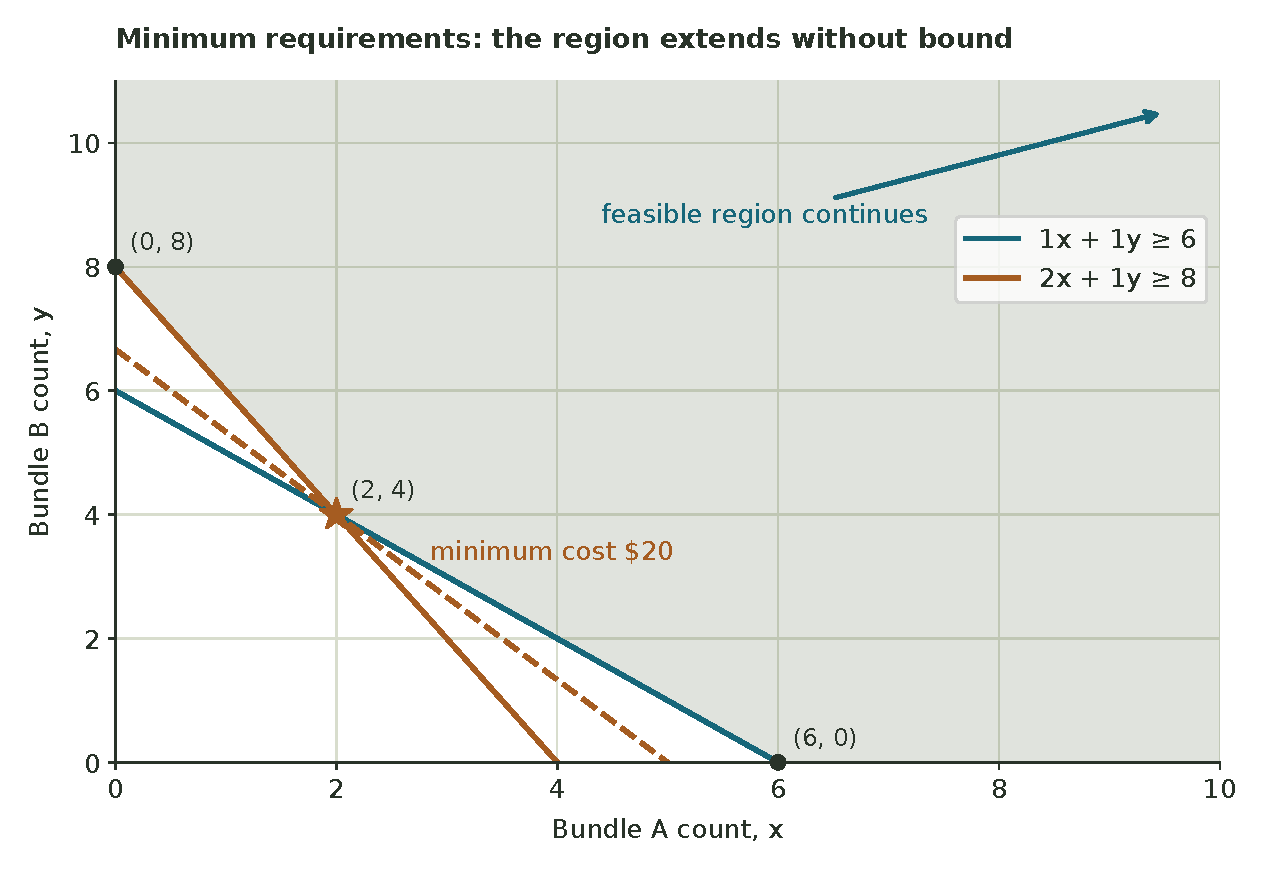
\includegraphics[width=\linewidth,height=3.2in,keepaspectratio]{../assets/week8/minimum-requirements.pdf}
\captionof*{figure}{The top and right edges of the picture are viewing limits, not extra constraints. The arrow shows the feasible region continuing. Buying more and more bundles raises this positive cost; it does not lower it indefinitely.}
\end{minipage}\par\medskip

\par\medskip{\small\renewcommand{\arraystretch}{1.35}\begin{tabularx}{\linewidth}{@{}YYYY@{}}\toprule
Boundary vertex & Notebooks & Pencils & Cost 4x+3y\\
\midrule
(0,8) & 8 & 8 & \$24\\
(2,4) & 6 & 8 & \$20\\
(6,0) & 6 & 12 & \$24\\
\bottomrule\end{tabularx}}\par\medskip


The minimum is \$20 at 2 A-bundles and 4 B-bundles. For this nonnegative-variable model, the least cost occurs at a feasible vertex. On an unbounded region, we must also check whether some allowed direction keeps improving the objective. Here all costs are positive, so going farther out cannot make the cost decrease forever.


The origin has cost zero but violates the supply requirements. This is why minimizing cost cannot be separated from stating what must be provided. If the only restrictions were upper limits and nonnegativity, doing nothing could indeed be the mathematical minimum-cost plan.



\begin{tcolorbox}[title={Pause and try 4},breakable]
Why is (0,6) not feasible for the supply order even though it provides all six notebooks?
\end{tcolorbox}


\Needspace{6\baselineskip}\section{A model can have a best plan, no plan, or no finite best value}


\par\medskip\noindent\begin{minipage}{\linewidth}
\centering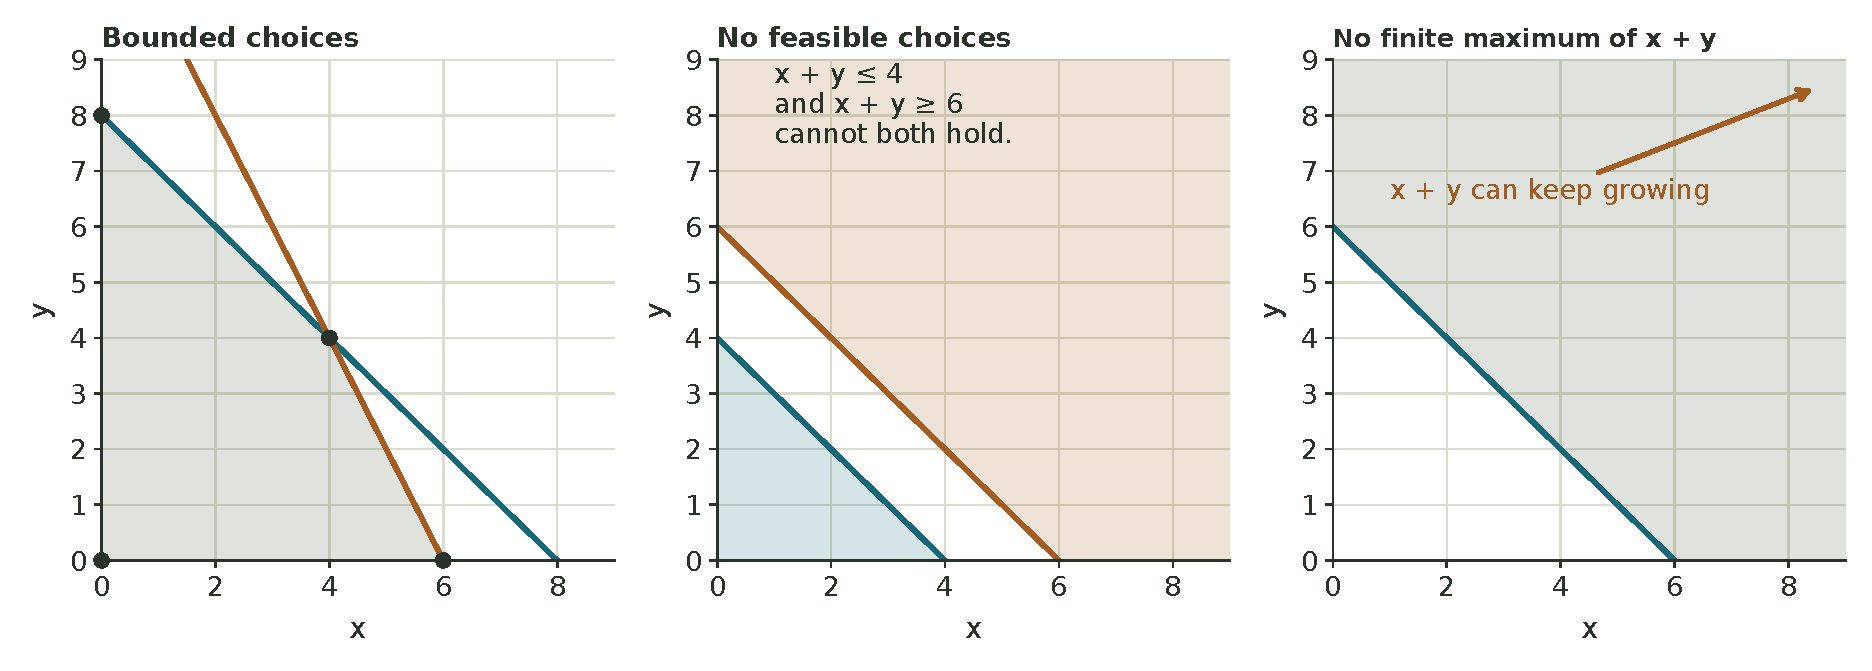
\includegraphics[width=\linewidth,height=3.2in,keepaspectratio]{../assets/week8/model-outcomes.pdf}
\captionof*{figure}{Separate the questions: Is any plan feasible? Is the region bounded? Can the objective keep improving without limit? An unbounded region can still have a finite minimum, as the supply-order example showed.}
\end{minipage}\par\medskip


\begin{itemize}
\item \emph{Infeasible model:} no point satisfies every constraint. For example, \(x+y\leq4\) and \(x+y\geq6\) cannot both hold. There is no permissible plan to optimize.
\item \emph{Unbounded objective:} feasible plans exist, but their scores improve without limit. For example, maximizing \(x+y\) with only \(x+y\geq6\) and nonnegativity allows arbitrarily large totals.
\item \emph{Finite optimum:} some feasible plan attains the best value. It may be one point, an edge, or a larger set when scores tie.

\end{itemize}

The optimizer identifies these different outcomes. It computes vertices from the actual constraints; a corner of its graph window is not automatically a real feasible vertex.


\begin{tcolorbox}[title={Included boundaries matter too},breakable,colback=warm,colbacktitle=warm,coltitle=gold,colframe=gold!35]

With \(0\leq x<1\), there is no largest allowable x: any proposed x can be increased a little while staying below 1. The value 1 is a limiting bound, but it is excluded. Our corner method uses non-strict inequalities so the relevant boundaries are available.


\end{tcolorbox}


\begin{tcolorbox}[title={Pause and try 5},breakable]
Does an unbounded feasible region always imply that there is no minimum? Give an example from this reading.
\end{tcolorbox}

\clearpage

\Needspace{6\baselineskip}\section*{Extension: whole-number plans}

Acres, mixture amounts, and hours can often be treated as divisible. Chairs, buses, and finished packs usually cannot. Requiring whole-number decisions adds an \emph{integer constraint}. It changes which points are allowed, even when the drawn continuous region stays the same.


\begin{tcolorbox}[title={Example \textperiodcentered{} Rounding can fail in two ways},breakable]

Maximize \(S=5x+8y\) subject to \(x+2y\leq8\), \(3x+2y\leq10\), and nonnegativity. The continuous best point is (1,3.5), with score \(5(1)+8(3.5)=33\).


Rounding up to (1,4) violates both limits: the totals become 9 and 11. Rounding down to (1,3) is feasible but scores only 29. The whole-number plan (0,4) is feasible and scores 32, so rounding down missed a better plan.


\end{tcolorbox}


\par\medskip\noindent\begin{minipage}{\linewidth}
\centering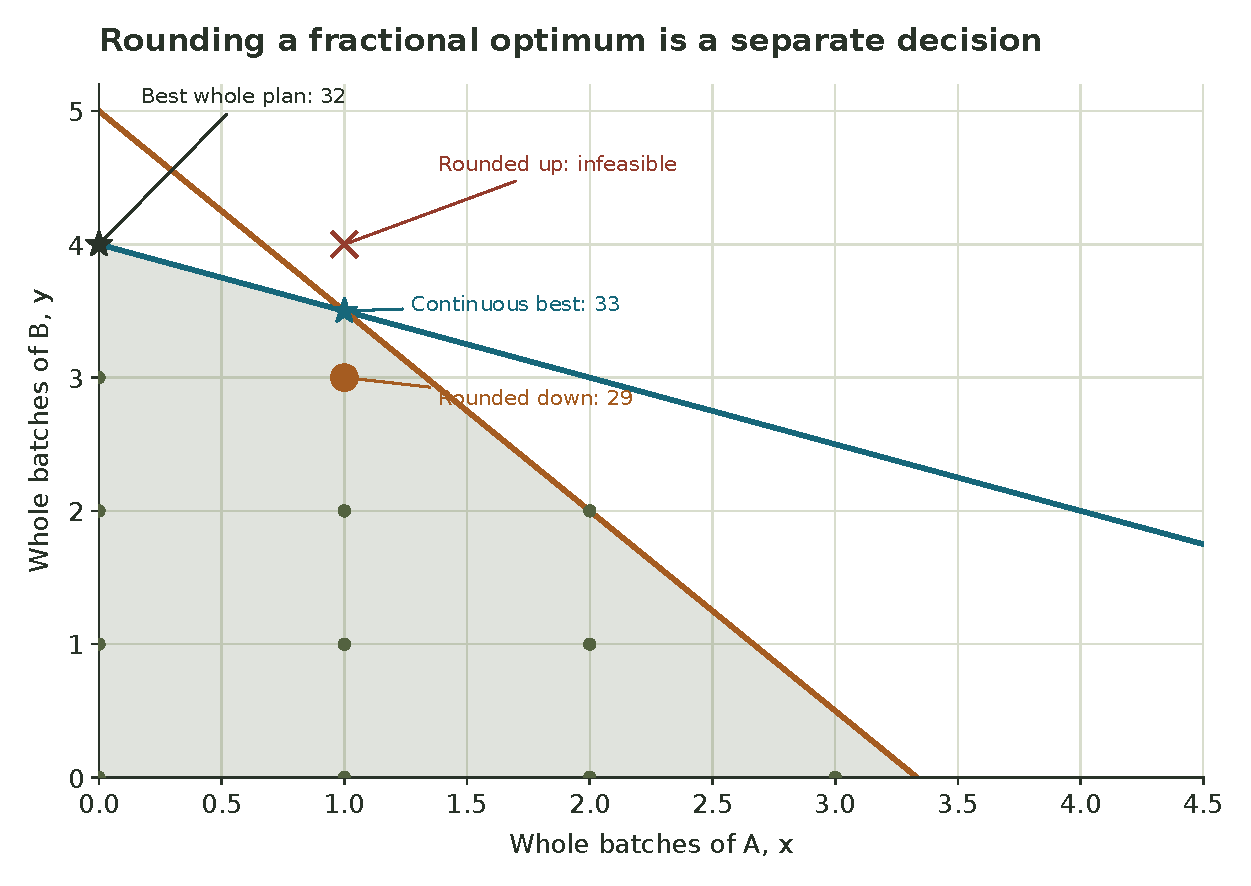
\includegraphics[width=\linewidth,height=3.8in,keepaspectratio]{../assets/week8/whole-number-plans.pdf}
\captionof*{figure}{For a small model, list feasible whole-number choices systematically. A fractional continuous optimum bounds the possible whole-number score from above, but it may not itself be usable.}
\end{minipage}\par\medskip


To verify the integer optimum here, try y = 0, 1, 2, 3, 4. The largest allowable whole x-values are 3, 2, 2, 1, 0, giving respective scores 15, 18, 26, 29, 32. This finite check establishes the best whole plan.



\begin{tcolorbox}[title={Pause and try 6},breakable]
What does the continuous maximum 33 establish about any feasible whole-number score in this example? Why does it not establish that 33 can be achieved with whole numbers?
\end{tcolorbox}

\clearpage

\Needspace{6\baselineskip}\section{A convex combination is a weighted average of points}

Weeks 2--3 used fractions, relative weights, and averages to summarize numbers. We can average points by averaging their coordinates. For points \(A=(2,1)\) and \(B=(8,5)\), use weights 0.75 and 0.25:

\[P=0.75A+0.25B=(0.75(2)+0.25(8),\;0.75(1)+0.25(5))=(3.5,2).\]
A \emph{convex combination} uses nonnegative weights that add to 1. For two points, all these combinations fill the segment between them. For three noncollinear points, they fill the triangle. The smallest convex set containing the given points is their \emph{convex hull}.



\par\medskip\noindent\begin{minipage}{\linewidth}
\centering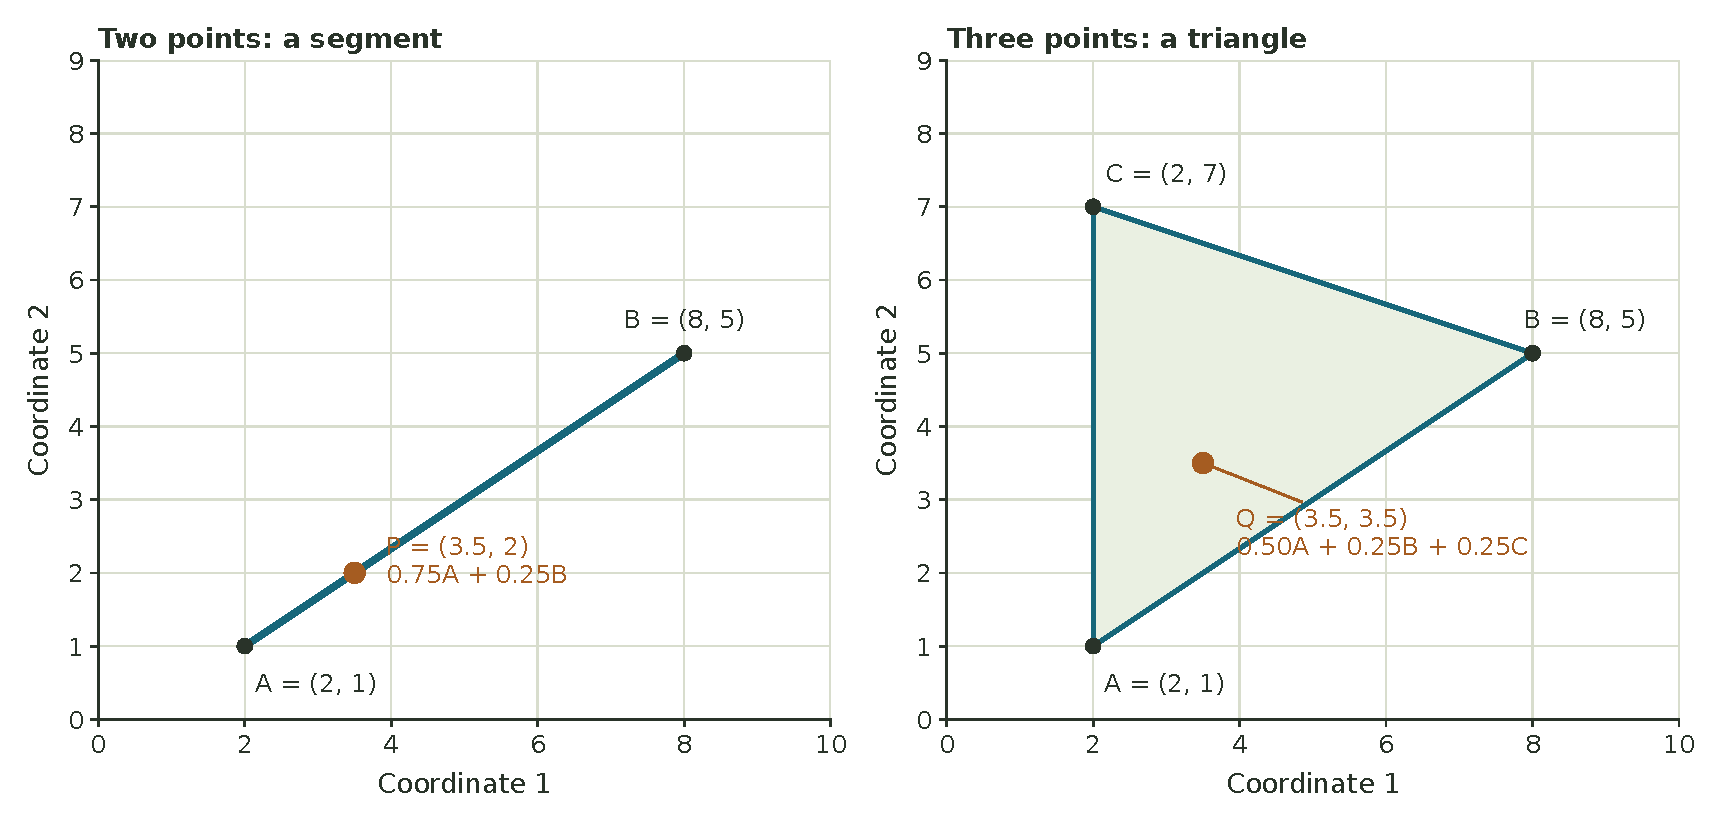
\includegraphics[width=\linewidth,height=3.2in,keepaspectratio]{../assets/week8/weighted-mixtures.pdf}
\captionof*{figure}{A weight of 0.75 on A places the result nearer A, one quarter of the way from A toward B. The numbers are coordinates in an invented representation; their axes have no assumed physical units.}
\end{minipage}\par\medskip


The AI application isolates one use of this idea: a normalized nonnegative weighted combination of value vectors in attention. The geometric guarantee concerns that one averaging step. Later transformations in a model need not stay in the original hull, and the weights do not certify that an interpretation is true.



\begin{tcolorbox}[title={Pause and try 7},breakable]
Why do weights 0.6 and 0.4 define a convex combination, while 1.2 and $-$0.2 do not?
\end{tcolorbox}


\Needspace{6\baselineskip}\section{A clear recommendation names its goal and assumptions}

Linear models assume constant rates: every extra pack uses the same resource amounts and adds the same contribution. They may omit bulk discounts, setup time, uncertain demand, waste, changing prices, staffing constraints, or a minimum service requirement. The graph is the consequence of those modeling choices.


Increasing a resource allowance in a ``$\le$'' constraint expands the feasible set or leaves it unchanged. Therefore the best maximum score cannot decrease. But it need not improve: another resource may still block every better plan. Tightening a limit can shrink the set or even make it empty.


\begin{tcolorbox}[title={Example \textperiodcentered{} More ingredients do not create more packing slots},breakable]

Keep \(x+y\leq8\), but increase the ingredient allowance from 12 to 16. All eight packs can now be type A: (8,0) uses 8 slots and 16 portions and contributes \$24. Increasing ingredients beyond 16 cannot improve this particular objective further while the eight-slot limit stays fixed: no pack contributes more than \$3, so eight packs can contribute at most \$24.


\end{tcolorbox}

\Needspace{5\baselineskip}\subsection*{A practical routine}

\begin{enumerate}
\item Define the decision variables, units, and whether fractions are meaningful.
\item Translate every resource limit and minimum requirement into a constraint.
\item State the objective and whether to maximize or minimize it.
\item Find all feasible vertices and check candidate intersections.
\item Compare objective values and identify ties or improving directions.
\item Check whole-number restrictions and interpret the plan and value.
\item Name a missing feature and explain what information would improve the model.

\end{enumerate}

Week 9 adds another reason a plan might be impossible: locations and resources must be connected by usable routes. Keep the same distinction there -- what is allowed, what is preferred, and what the model leaves out.


\clearpage
\section*{Further Worked Models}
\subsection*{Furniture: compare every feasible corner}
A furniture maker produces chairs $x$ and desks $y$ per week. Two resource constraints are $2x+3y\leq120$ and $x+2y\leq70$, with nonnegativity. Maximize contribution $P=40x+70y$.

The first boundary has intercepts $(60,0)$ and $(0,40)$; the second has $(70,0)$ and $(0,35)$. The tighter axis limits give $(60,0)$ and $(0,35)$. To find the non-axis intersection, double $x+2y=70$ and subtract $2x+3y=120$: $y=20$, then $x=30$.

{\renewcommand{\arraystretch}{1.35}\begin{tabularx}{\linewidth}{@{}YYYY@{}}\toprule
Corner & First resource & Second resource & Contribution\\\midrule
$(0,0)$ & 0 & 0 & \$0\\
$(60,0)$ & 120 & 60 & \$2,400\\
$(30,20)$ & 120 & 70 & \$2,600\\
$(0,35)$ & 105 & 70 & \$2,450\\\bottomrule
\end{tabularx}}

All four corners pass both limits. The maximum is \$2,600 at 30 chairs and 20 desks. The plan and its value are different quantities; both belong in the recommendation.

\subsection*{A resource limit can be redundant}
Suppose a different model has limits $x+2y\leq20$ and $x+2y\leq24$. Every point passing the first also passes the second. The second is redundant. This differs from merely having slack at one plan: a constraint can be slack at a particular optimum yet still exclude other choices elsewhere.

\clearpage
\subsection*{A third real constraint can create a fifth corner}
A print shop has three limits:
\[
x+2y\leq60,\quad x+y\leq40,\quad2x+y\leq70,\quad x,y\geq0.
\]
Here $x$ counts posters and $y$ banners. Maximize the invented contribution $P=15x+35y$.

Intersect the first two non-axis boundaries to get $(20,20)$; the third total is 60, so it passes. Intersect the second and third to get $(30,10)$; the first total is 50, so it passes. The first and third meet at $(80/3,50/3)$, but this candidate has $x+y=130/3>40$, so it must be discarded.

The x-axis corner is $(35,0)$: the third constraint is tighter there than the other two. The y-axis corner is $(0,30)$: the first constraint is tighter there. Together with the origin and the two valid non-axis intersections, these give five corners.

{\renewcommand{\arraystretch}{1.35}\begin{tabularx}{\linewidth}{@{}YYY@{}}\toprule
Feasible corner & Calculation & Contribution\\\midrule
$(0,0)$ & $15(0)+35(0)$ & \$0\\
$(35,0)$ & $15(35)+35(0)$ & \$525\\
$(30,10)$ & $15(30)+35(10)$ & \$800\\
$(20,20)$ & $15(20)+35(20)$ & \$1,000\\
$(0,30)$ & $15(0)+35(30)$ & \$1,050\\\bottomrule
\end{tabularx}}

The maximum is \$1,050 at $(0,30)$. All three resource constraints matter to this feasible region; none is redundant. A calculation at a visually prominent intersection, such as $(20,20)$, is not a substitute for comparing all corners.

\begin{tcolorbox}[title={A useful distinction}]
A constraint is \emph{binding at a plan} when it holds with equality there. It is \emph{redundant in a model} when removing it leaves the entire feasible set unchanged. These are different claims.
\end{tcolorbox}

\clearpage
\section*{Part II Review}
Use nonnegative variables and included boundaries. Show a corner table or explicit calculation and report both a plan and its objective value.
\begin{enumerate}
\item For the club's corners $(0,0),(6,0),(4,4),(0,8)$, maximize $P=3x+2y$. What is the minimum if there is no lower production requirement?
\item On the same region, maximize $R=x+4y$ and then $T=x+y$. Describe the complete optimal edge for $T$, including its whole-number points.
\item Maximize $f=5x+8y$ subject to $x+2y\leq16$, $3x+2y\leq24$. Find all corners and compare. Check resource use at the best plan.
\item Minimize $C=3x+5y$ subject to $x+y\geq8$, $2x+y\geq10$. Find the boundary vertices. Explain why the mixed boundary intersection is not automatically best.
\item For the furniture model in the worked example, compare the best plan with producing only desks. Does the higher per-item contribution determine the answer by itself?
\item For the three-limit print shop, why is $(80/3,50/3)$ not a feasible corner? Which corner maximizes $15x+35y$?
\item A toy workshop has $3x+y\leq120$, $x+2y\leq80$, and contribution $P=8x+5y$. Find the corners and best plan. Then change the contribution to $5x+8y$ and compare.
\item A municipality divides an invented \$500-thousand budget between roads $x$ and parks $y$, measured in thousands of dollars. Require $x\geq100$, $y\geq80$, $x+y\leq500$. Maximize an invented score $S=3x+4y$. What does the score leave for people to decide?
\item A polygon has corners $(0,0),(8,0),(5,4),(0,6)$. For cost $C=4x+6y$, which of the three listed nonzero corners is cheapest? Why is that not the minimum over the full polygon? Give a different positive feasible plan with lower cost.
\item For $x+2y\leq8$, $3x+2y\leq10$, maximize $5x+8y$ continuously and then using whole numbers. Check rounding up and rounding down from the continuous best point.
\item Compute $0.75A+0.25B$ for $A=(2,1),B=(8,5)$. Add $C=(2,7)$ and normalize amounts $2,1,1$. Where do the resulting points lie? Why do weights $1.2,-0.2$ fail the convex-combination test?
\item Explain the difference between an infeasible model and an unbounded objective. Give an example of an unbounded region with a finite minimum. Explain why $0\leq x<1$ has no largest allowable x.
\item Keep $x+y\leq8$ and increase the club's ingredient allowance from 12 to 16, then 20. Maximize $3x+2y$ at each stage. Why does the extra ingredient allowance eventually stop helping?
\item Recommend a plan for the original chair-and-table workshop with wood limit 40, assembly limit 14, and contribution $30x+50y$. Use resource totals and a comparison with another feasible plan. Name a relevant missing feature.
\end{enumerate}

\clearpage
{\setlength{\parskip}{4pt}\setlist{itemsep=4pt,topsep=3pt}\titlespacing*{\paragraph}{0pt}{5pt}{.75em}
\section*{Solutions and Reasoning}

\paragraph{Short check 1.}
P=3(2)+2(5)=16. The score alone does not prove feasibility; check the constraints. Here packing uses 7 and ingredients use 9, so the plan is feasible.


\paragraph{Short check 2.}
The best corner can occur where two non-axis boundaries meet. Here (4,4) gives \$20, exceeding the \$18 and \$16 at the axis corners. The method requires every feasible vertex.


\paragraph{Short check 3.}
Every point on the edge joining two optimal adjacent vertices has the same maximum score. Equal scores alone do not establish optimality: some other vertex might score higher. First compare all feasible corners.


\paragraph{Short check 4.}
It supplies only 6 pencils, below the minimum 8. Both requirements must hold. A boundary intercept of one requirement may fail another.


\paragraph{Short check 5.}
No. The supply-order region extends indefinitely, but positive costs give a minimum of \$20 at (2,4). Unbounded choices and an unbounded objective are different properties.


\paragraph{Short check 6.}
Every whole-number feasible plan is also continuously feasible, so its score is at most 33. But the point giving 33 has a fractional coordinate, so it does not establish an attainable whole-number score.


\paragraph{Short check 7.}
The first pair is nonnegative and sums to 1. The second also sums to 1 but has a negative weight; it can extrapolate beyond the segment. Both conditions are needed.



\subsection*{Part II Review: solutions}
\begin{enumerate}
\item Corner values are $0,18,20,16$. Maximum \$20 is at $(4,4)$. With only upper limits and nonnegativity, minimum contribution is 0 at zero production. A minimum-cost model may need minimum service requirements.
\item R-values are $0,6,20,32$, so $(0,8)$ is best. T reaches 8 along the edge from $(4,4)$ to $(0,8)$. Its whole-number plans are $(0,8),(1,7),(2,6),(3,5),(4,4)$.
\item Subtraction gives $x=4,y=6$. Corners are $(0,0),(8,0),(4,6),(0,8)$; scores are $0,40,68,64$. The maximum is 68 at $(4,6)$, using 16 units of the first resource and 24 of the second.
\item Corners are $(8,0),(2,6),(0,10)$, with costs $24,36,50$. The minimum is 24 at $(8,0)$. It provides 8 of the first requirement and 16 of the second, exceeding its 10-unit minimum by 6. A feasible axis corner can outperform a mixed intersection.
\item $(30,20)$ gives \$2,600; desks only gives $(0,35)$ and \$2,450. The best mix depends on both resource limits, not just the larger contribution per item.
\item That intersection has $x+y=130/3>40$ and violates the middle constraint. The maximum is \$1,050 at $(0,30)$, which passes all three limits.
\item Corners are $(0,0),(40,0),(32,24),(0,40)$. Original scores are $0,320,376,200$, so $(32,24)$ is best at 376. Under $5x+8y$, scores are $0,200,352,320$; the same plan remains best but its score changes. Changing an objective need not always move the optimum.
\item Corners are $(100,80),(420,80),(100,400)$. Scores are $620,1580,1900$. The score selects roads \$100,000 and parks \$400,000. Its coefficients and minimum allocations are modeling choices, not facts establishing what a community ought to value.
\item The three costs are 32,44,36, so $(8,0)$ is cheapest among those candidates. The full polygon includes $(0,0)$ at cost 0 and, for example, $(1,0)$ at cost 4. A real production floor needs an explicit constraint, not deletion of one point.
\item Continuous maximum 33 is at $(1,3.5)$. Rounding up to $(1,4)$ gives resource totals 9 and 11, both too large. Rounding down to $(1,3)$ is feasible but scores 29. The best whole plan is $(0,4)$ at 32; enumerate y-values 0--4 to verify.
\item The first point is $(3.5,2)$, on the A--B segment. Normalized amounts give weights $(0.5,0.25,0.25)$ and point $(3.5,3.5)$ inside the triangle. A negative weight violates nonnegativity even if the weights sum to 1.
\item Infeasible means no plan satisfies every condition. Unbounded objective means feasible plans improve the score without finite limit. The supply-order model $x+y\geq6$, $2x+y\geq8$ has unbounded choices but minimum $4x+3y=20$ at $(2,4)$. Under $0\leq x<1$, any allowed x can be increased while remaining below 1; the limiting bound 1 is excluded.
\item With allowance 12, the maximum is 20 at $(4,4)$. At 16 and 20, it is 24 at $(8,0)$. The packing limit permits at most eight packs, and each contributes at most 3; no plan can exceed 24 while that limit stays fixed. Beyond 16, the ingredient constraint is redundant.
\item Produce 8 chairs and 6 tables: wood use $2(8)+4(6)=40$, assembly use $8+6=14$, contribution \$540. Ten tables alone are feasible but contribute \$500. Demand, waste, setup time, resource uncertainty, and variable production rates are examples of missing features that could change a real recommendation.
\end{enumerate}
\subsection*{Optional primary source for the AI connection}
Vaswani et al., \href{https://arxiv.org/html/1706.03762v7#S3.SS2}{\emph{Attention Is All You Need}, Section 3.2}. The geometry applies to the normalized weighted value combination at that step; later transformations can move a representation beyond the original hull. The vectors and weights in this unit are constructed examples.
}
\end{document}
